%!TEX root = ../thesis.tex

\chapter{Technologies}\label{chapter:technologies}











































% TODO mettere da qualche parte overview of underlaying network technologies

% Hardware Addressing Schemes

To fully understand the project and the choices behind it, is worth taking a look at some backgrounds technology which can be useful to know before proceeding further into this thesis.
In this chapter we describe DTNs, the notion of peer-to-peer and overlay networks.

internetworking \cite{internetworking}

% TODO andare a recuperare dal libro di douglas
\section{Approaches To Network Communication}

connection oriented vs connectionless

Despite the potential drawback of not being able to guarantee network capacity,
connectionless networks have become extremely popular.

WAN vs LAN

WAN technologies, sometimes called long haul networks, provide communication
over long distances.

LAN technologies provide the highest speed connections among computers, but
sacrifice the ability to span long distances.

Instead, vendors apply the terms loosely to help customers distinguish among technologies.

\section{Radio technologies}\label{sec:section_two}

In order to give a complete picture of radio transmitting technologies, it is important to make a distinction among the ones that are made for internal or nearby use vs the ones that are used for longer distances.

% TODO spiegare LAN, MAN, WAN

With new transmission technologies, new network architectures have emerged

% TODO spiegare LPWAN

Distinction of low cost vs higher cost
% http://iotfactory.eu/iot-knowledge-center/overview-of-iot-networks/

\begin{figure}
	\centering
	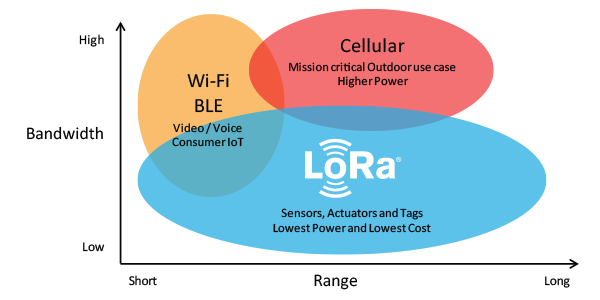
\includegraphics[width=\textwidth]{resources/img/LoRa_Why_Range}
	\caption{}
\end{figure}

% PAPER : LPWAN Technologies: Emerging ApplicationCharacteristics, Requirements, andDesign Considerations
\begin{figure}
	\centering
	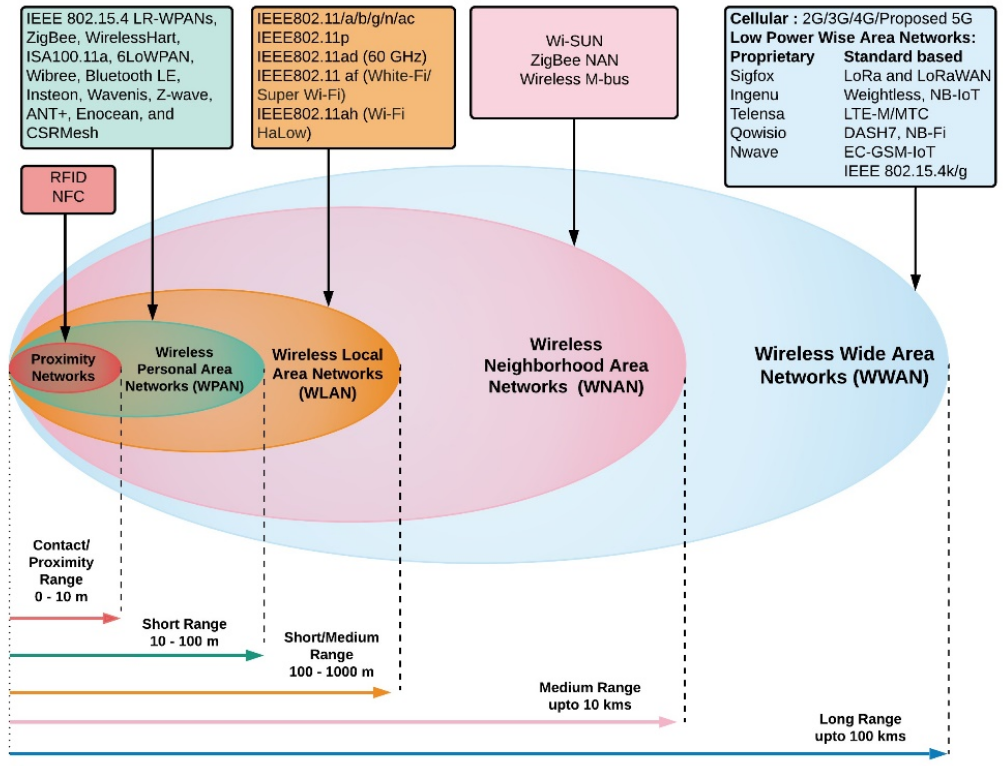
\includegraphics[height=\textwidth, angle=90]{resources/img/iot_range}
	\caption{}
\end{figure}

\subsection{LoRa}

https://lora-alliance.org/

https://www.semtech.com/lora

\subsection{LoRaWAN}

\subsection{Bluetooth}		

\subsection{WiFi}



IEEE 802.11, better known in the public as WiFi, short for wireless fidelity

\subsection{LTE}



\section{LoRa and LoRaWAN}

\section{Hardware (Microcontrollers)}

	Microcontrollers (or MCUs) are compact integrated circuits designed to govern a specific operation in an embedded system.
	
	Devices and CPUs have become smaller and more granular, allowing to have simple micro computers that need very little power resources, both computational and battery, that they can be used for very specific functions.
	
	Some examples can be:
	\begin{itemize}
		\item smog detector, which sounds an alarm when excess smog is sensed
		\item car range detector, that sends an alarm to the car's braking system when there is an object in front of it
		\item etc.
	\end{itemize}

\subsection{Arduino}

	% https://www.arduino.cc/en/Main/AboutUs
	

\subsection{Raspberry Pi}

\noindent
\begin{minipage}{0.5\textwidth}% adapt widths of minipages to your needs
	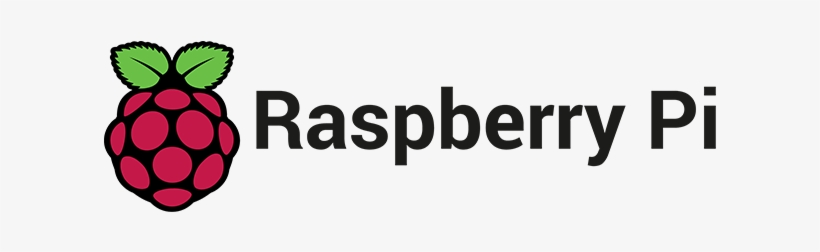
\includegraphics[width=\textwidth]{resources/img/51-513503_pi-raspberry-pi-logo}
	\captionof{figure}{\textit{Pycom} company logo}
\end{minipage}%
\hfill%
\begin{minipage}{0.55\textwidth}\raggedright
	Yesterday,\\
	all my troubles seemed so far away\\
	Now it looks as though they're here to stay\\
	Oh, I believe in yesterday.				Yesterday,\\
	all my troubles seemed so far away\\
	Now it looks as though they're here to stay\\
\end{minipage}	

\subsection{Pycom}

\noindent
\begin{minipage}{0.5\textwidth}% adapt widths of minipages to your needs
	
\includegraphics[width=\textwidth]{resources/img/pycom-logo-new-rp1}
	\captionof{figure}{\textit{Pycom} company logo}
\end{minipage}%
\hfill%
\begin{minipage}{0.55\textwidth}\raggedright
	Yesterday,\\
	all my troubles seemed so far away\\
	Now it looks as though they're here to stay\\
	Oh, I believe in yesterday.				Yesterday,\\
	all my troubles seemed so far away\\
	Now it looks as though they're here to stay\\
\end{minipage}

A Pycom development board has considerably more I/O than a standard Arduino, but probably comparable to an Arduino Mega. Easy to program via Python. Good example code from Pycom. Small community. Low cost. Not at all comparable to Raspberry Pi in terms of software flexibility.

% https://www.reddit.com/r/IOT/comments/kx6knr/what_do_people_think_of_pycom_products/
A complete LoRa gateway (Pygate + WiPy + IP67 box + antenna) costs around \$100, which is pretty good. So far very stable, and it was easy to configure. There's a PoE unit, but I use WiFi (at my home).

% TODO ADD TO REFERENCES
% https://docs.pycom.io/gitbook/assets/lopy4-pinout.pdf
